\documentclass[12pt]{article}

% packages
\usepackage[utf8]{inputenc}
\usepackage{graphicx}
\usepackage{subcaption}
\usepackage[
top=2cm,
bottom=2cm,
left=2cm,
right=2cm,
headheight=17pt, % as per the warning by fancyhdr
includehead,includefoot,
heightrounded, % to avoid spurious underfull messages
]{geometry} 
\usepackage{amsmath,amssymb}
\usepackage{fancyhdr}
\usepackage{titling}
\usepackage[style=ieee, backend=bibtex]{biblatex}
% paragraph indentation
\usepackage{indentfirst}
\setlength{\parindent}{2em}
% page style
\pagestyle{fancy}
% section name without number
\renewcommand{\sectionmark}[1]{\markright{#1}}
\renewcommand{\subsectionmark}[1]{}
% header and footer lines
\renewcommand{\headrulewidth}{1.5pt}
\renewcommand{\footrulewidth}{1.5pt}
% line spacing
\renewcommand{\baselinestretch}{1.5} 
% \fancyheadoffset{1 cm} 
\fancyhead[L]{A Computational Model of the Islets of Langerhans}
\fancyhead[R]{\rightmark}
\fancyfoot{}
\fancyfoot[R]{\thepage}
\fancyfoot[L]{UF CISE}
\fancyfoot[C]{Tikahari Khanal}


% references
\addbibresource{ref.bib}
% title
\title{
{A Computational Model of the Islets of Langerhans}\\
{\large University of Florida\\ Department of Computer and Information Science and Engineering}
}
\author{Tikahari Khanal}

% document
\begin{document}
\begin{titlingpage}\setlength{\droptitle}{30pt} % lower the title
	\maketitle
	\begin{abstract}
	The pancreas plays a vital role in the regulation of blood glucose, metabolism, and digestion. Endocrine cells of the pancreas, which secrete the major hormones responsible for glucose regulation, exhibit characteristic electrophysiological excitability similar to what is observed in neurons. This electrical excitability and the relevant metabolic pathways involved can be considered thermodynamic processes and subsequently mathematically modeled according to the temporal dynamics of relevant ion channels and the enthalpies of the corresponding reactants and products. Such a mathematical model can yield information otherwise impossible to discern in vivo and facilitate greater efficacy of drug and treatment development. In this thesis, we seek to develop an ensemble model of endocrine cells of the pancreas parameterized through a single-objective evolutionary algorithm.
	\end{abstract}
\end{titlingpage}

\tableofcontents
\newpage
\renewcommand{\listfigurename}{Figures}
\listoffigures
\newpage

\section{Background}
\subsection{Pancreas}
The pancreas is commonly associated with the production of insulin and its subsequent effect on the uptake and metabolic degradation of glucose \cite{caicedo_paracrine_2013}. This function has major implications for research into disorders associated with a malfunction in the production of or response to insulin (i.e. obesity, diabetes, metabolic syndrome, etc.) and has guided much of the clinical and computational research into the structure and function of the organ \cite{woods_pancreatic_2006}. The pancreas, however, is responsible for producing a broad range of hormones and enzymes and is implicated in a considerable scope of metabolic processes. It can be thought of as an ecosystem with characteristic spatial, physiological, and environmental profiles that themselves exist in a compelling purview of phenotypes. 
\par Less frequently considered but biologically essential roles include the production of digestive enzymes, the release of neurotransmitters, and feedback regulation of major metabolic pathways. Digestive enzymes critical to peptide and saccharide breakdown include chymotrypsin, trypsin, pepsin, lipase, and pancreatic amylase and are released by acinar cells (exocrine cells of the pancreas) \cite{ianiro_digestive_2016}. The pancreas is, intuitively, the site of origin for the pancreatic duct where bicarbonate is released as a response to the presence of chyme in the duodenum \cite{hegyi_pancreatic_2011}. Further, recent research on human islets has revealed that gamma aminobutyric acid (GABA), a neurotransmitter associated with an inhibitory effect on the central and peripheral nervous systems, is released by $\beta$ cells \cite{rutter_gaba_2017}. A similar study on mouse islets has found that endocrine cells of islets express the genes implicated in the production of serotonin and respond to the presence of the neurotransmitter through a decreased insulin production \cite{chandra_neural_2009}.
\par The human pancreas sits in the posterior abdomen wall with an average weight of approximately 90 grams. It is derived from embryonic endoderm tissue and can be divided into at least four structurally distinct segments: the head, body, tail, and uncinate process \cite{g_quantification_2012} \cite{birnbaum_head_2019}.
\par Endocrine cells of the pancreas occuppy 1-2 \% of the pancreas by mass and can be divided into three types, often categorized by a characteristic secretagogue \cite{pour_are_2002}. They exist within islets (Islets of Langerhans) and can be found in clumps of between 70 to over 100 cells. $\alpha$ cells are known for secreting glucagon which is associated with low blood glucose and responsible for stimulating the release of glucose from cells, gluconeogenesis, and the breakdown of fatty acid and saccharide energy stores \cite{jiang_glucagon_2003}. $\beta$ cells are make up the highest percentage of endocrine cells within the islet and are known for producing and secreting insulin \cite{g_quantification_2012}. Insulin is often thought of as complementary to glucagon since it is associated with high blood glucose and stimulates its uptake from the blood, glycolysis, and the synthesis of fatty acid and saccharide energy stores \cite{hatting_insulin_2018}. $\delta$ cells are the least well studied and common of the major endocrine cells of the pancreas \cite{vergari_somatostatin_2020}. They secrete somatostatin, which affects cell proliferation, neurotransmission, and the release of glucagon and insulin from the aforementioned $\alpha$ and $\beta$ cells \cite{braun_somatostatin_2009}. $\epsilon$ cells comprise a very small percentage of islet cells and are responsible for the release of the hormone ghrelin, which most strongly associated with the regulation of hunger \cite{sakata_development_2019}.
\par Electrical activity in these endocrine cells is a product of the flow of various ion species across their respective electrochemical gradients \cite{riz_mathematical_2014}. These ions flow through protein channels with different gating properties (i.e. voltage-dependent, pH-dependent, substrate-dependent, etc.) and are responsible for changes in membrane potential or enzymatic cascades that facilitate communication between cells, tissues, and organs. 
\par The Zhang-Liu hypothesis outlines the biological basis of electrical excitability in $\beta$ cells and has recently been generalized to $\alpha$ and $\delta$ cells \cite{briant_functional_2017}. According to this hypothesis, electrical activity is stimulated by the intake of glucose, which after degradation through glycolysis and further processing in the Kreb's Cycle, yields an increase in cyptoplasmic adenosine triphosphate (ATP). This closes ATP-dependent potassium channels and causes an initial increase in membrane potential. The change in membrane potential, in turn, results in the opening of voltage-dependent calcium channels and the intake of calcium. This current drives a spike and the influx of calcium activates various secondary messenger pathways that lead to hormone secretion.
\subsection{Modeling Electrophysiology}
The electrical excitability of neurons has long been observed, but until the mid 20th century the mechanisms behind this behavior were poorly understood. In 1952, A.L Hodgkin and A.F. Huxley released a nobel prize winning series of papers in which they developed a mathematical model that elucidated the principles of ion channel dynamics in the giant squid axon \cite{hodgkin_effect_1949}. Modern modeling of electrically excitable membranes takes its root in these papers and often includes some combination of the following equations which constituted their mathematical model \cite{riz_mathematical_2014}.
\begin{figure}[h!]\label{circ}
	\centering
	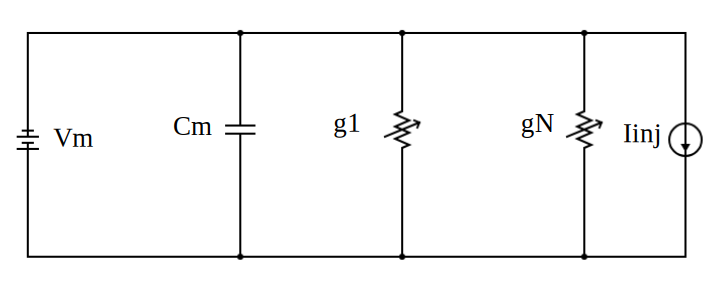
\includegraphics[scale=0.65]{Figures/circuit_labeled.png}
	\caption{Membrane as a circuit}
\end{figure}
\begin{equation}\label{hh}
\frac{dV_m}{dt} = \frac{1}{C_m} (I_{inj} - \bar{g}_k n^4 (V_m - V_k) -\bar{g}_{na} m^3 h (V_m - V_{na}) - \bar{g}_l (V_m - V_l))
\end{equation}
\begin{equation}\label{dn}
\frac{dn}{dt} = \alpha_n (V_m) (1 - n) - \beta_n (V_m) n
\end{equation}
\begin{equation}\label{dm}
\frac{dm}{dt} = \alpha_m (V_m) (1 - m) - \beta_m (V_m) m
\end{equation}
\begin{equation}\label{dh}
\frac{dh}{dt} = \alpha_h (V_m) (1 - h) - \beta_h (V_m) h
\end{equation}

\par Their first major breakthrough came in the form of an assumption; that the lipid bilayer and protein channels of the axon were analogous to capacitive and resistive elements of a circuit (see Figure 1). This circuit is subject to the same laws that would govern the flow of current if it ws to take a physical form, and thus, by Ohm's Law and Kirkoff's Second Law, equation \ref{hh} can be derived. It is worth noting that the membrane potential corresponding to an electromotive force in the equivalent circuit is determined by the various electrochemical gradients across the cell's membrane and can be quantified by a modified form of the Nernst Equation (equation \ref{Nernst}). 
\begin{equation}\label{Nernst}
E = -\frac{RT}{nF} \ln Q
\end{equation}
\par Their second major breakthrough was that ion channel permeability (represented in equation \ref{hh} as the term multiplied against the membrane potential and reversal potential: i.e. $\bar{g}_k n^4$ for the sodium channel) was dependent on membrane potential and its own state. This temporal relationship between permeability and membrane potential was represented through a series of differential equations wherein the rate of activation ($\alpha_m$) is multiplied by the proportion of closed channels and the rate of inactivation ($\beta_m$) is similarly multiplied by the proportion of open channels. These rates were modeled by the Boltzmann distribution and had to be experimentally determined.
\begin{equation}
\frac{P_o}{P_c}  = K e^{qV}
\end{equation}
\par In the above equation, the ratio of the probability of an ion channel taking an open state to the same ion channel taking a closed state is equal to the free energy difference between those states. This is determined by a modified form of Gibb's Free Energy equation ($\Delta G = -qVln(K)$). By solving for the probability of an open channel we can derive an equation similar of form to that used to represent the rate of opening of a (potassium) channel in the original Hodgkin and Huxley model (equation \ref{hhn}).
\begin{equation}
P_o = \frac{1}{1 + \frac{e^{-qV}}{K}}
\end{equation}
\begin{equation}\label{hhn}
\alpha_{n} = \frac{0.1(10-V_m)}{e^{\frac{10-V_m}{10}}-1}
\end{equation}
\subsection{Modeling Diffusion}
Many biological processes which researchers have attempted to transcribe into a computational form involve the release and uptake of various hormones across dynamic gradients (i.e. electrochemical). Often the molecules being transferred from one location to another are transformed from one state to another either by means of a reaction with a similar molecule undergoing an analogous pattern of uptake and release or by means of an enzyme in a catalytic process. Since the molecules of interest often react with each other and form an intricate system of diffusion gradients and chemical reactions, these components of computational models of such biological systems are bundled together and represented through a single system of equations known as the Kolmogorov–Petrovsky–Piskunov system (or more simply: the reaction-diffusion system) \cite{fisher_wave_1937}.
\begin{equation}\label{rxd}
\delta_t u = D \delta_x^2 u+R(u)
\end{equation}
\par In this equation, $u$ represents some macroscopic variable such as concentration or mole fraction, $D$ a diffusion coefficient, $\delta_x^2 u$ diffusion, and $R(u)$ some reaction that affects a change in $u$. This system is often used when modeling pattern formation or the equilibrium of a system involving multiple ion species \cite{kondo_reaction-diffusion_2010}. Within the context of modeling cells, reaction diffusion allows researchers to predict the path of individual ions through extracellular spaces and their general flow from one cell to another.
\subsection{Previous Models}
The development and refinement of computational models of the pancreas has been a field of interest since at least the early 1980s \cite{chay_minimal_1983}. However, much of the research in this field during this period involved investigations into the function of beta cells often without consideration of the other major endocrine cells, even excluding the effect those cells may have on beta cell function. This is understandable as the role of beta cells in the production of insulin and its association with diabetes and obesity have been long understood and observed. However, the growing body of knowledge in the field points to islets being intricate systems of endocrine cells whose form and function are best understood through their role in macro level functions of the pancreas.
\par Recently, models have refined the previous work done on islets through wider scopes of considered cells and biological processes, more rigidly determined experimental constants, and the use of more considerable hardware resources that allow for simulations with greater space and time complexity. This work will define the outline of the model developed in this thesis and includes a model of $\beta$ cells by Fridlyand and models of $\alpha$ and $\delta$ cells by Watts and Sherman \cite{fridlyand_pancreatic_2016} \cite{watts_modeling_2014}. It is worth noting that these models differ in scope, with the computational models of $\alpha$ and $\delta$ cells accounting for the production and degradation of various intermediates in metabolic pathways leading to exocytosis while the computational model of $\beta$ cells focuses only on variables directly related to changes in membrane potential.

\section{Computational Model}
\subsection{Overview}
This thesis involved two major components: simulations of islet instances and an evolutionary algorithm which would score, manipulate, and select superior models with some randomization from those simulations. These components involved differences in requisite hardware resources, data processing, and general purpose and thus were executed and developed separately. In this section we consider the reasoning behind choices made regarding the simulations of islet instances.
\subsection{Framework}
NEURON, a set of language and libraries that facilitate the development of computational models of electrically excitable cells made public by the Yale School of Medicine \cite{hines_neuron_1997}, was selected to create and solve the previously mentioned systems of reaction-diffusion and circuit equations. These systems of equations were represented in nmodl, transpiled to c, and called from within a python script to minimize the space and time complexity of what would have been the most computationally expensive portion of the project  \cite{hines_expanding_2000}. NEURON also presented an array of differential equation solvers with varying stabilities and error bounds; for this implementation, the \emph{Cnexp} solver was selected since it is the recommended solver for Hodgkin-Huxley style models and able to solve stiff systems with up to second-order accuracy.
\par In order to best navigate the volume of data produced by these simulations and the significance of subtleties therein, the executables were written in python and dispatched in the University of Florida's high performance computing environment (Hipergator). This allowed for the storage of 10 TB of data on disk, access to over 128 GB of memory, the use of popular and effective packages for scientific computing (i.e. numpy, scipy, etc.), and the eventual parallelization of the evolutionary algorithm (see the Architecture section for more details).
\subsection{Physiological Properties}
Hodgkin-Huxley style models of electrically excitable cells developed with NEURON determine changes in a cell's membrane potential through calculations done on separate currents corresponding to unique ion species. These currents were calculated using properties of ion channels which were represented in nmodl and added to the cell object provided by the framework. This cell object was then added to the space in which the simulation takes place and the values associated with its mechanisms recorded. 
\par All cells contained sodium and potassium ion channels which were represented through the standard Hogdkin-Huxley style gating variables and experimentally determined rate functions. All cells also contained low and high (L and T type, respectively) voltage gated calcium channels with $\alpha$ and $\delta$ cells incorporating a PQ type (high voltage gated channels commonly associated with purkinje fibers) channel \cite{hashimoto_postsynaptic_2011}. Other currents which were not associated with a single protein channel that were considered in the model include but are not limited to a delayed rectifying potassium current (KDR), an ATP-dependent potassium current (KATP), a G-protein inward rectifying potassium current (GIRK), a GABA current, a background potassium current, and a background sodium current. Leak channels were also included in all cells to represent ion flow through perforations in the lipid membrane. 
\par Hormone secretion was modeled differently in $\beta$ cells than in $\alpha$ and $\delta$ cells. In $\beta$ cells, insulin release was considered only in the context of a cyptoplasmic calcium pool while glucagon and somatostatin release in $\alpha$ and $\delta$ cells were considered in the context of priming and depriming factors that attempted to represent exocytosis on the level of individual granules.

\subsection{Connectivity}
It is widely recognized that the major endocrine cells of the pancreas ($\alpha$, $\beta$, $\delta$) coregulate one another through their characteristic secratogogues. Although considerable regulation of peer endocrine cells can be an effect of downstream metabolic pathways stimulated by a secretory molecule, to maintain consistency and simplicity in this model's implementation, only insulin, glucagon, somatostatin, and GABA were considered as having an effect on other cells. That effect was limited to changing secretion rates of characteristic secratogogues and the conductance of the KATP and  GIRK ion channels in the cells that contained them.
\par A unique aspect of this model is that cells are connected according to their spatial distribution and their interaction governed by secretory agents within the previously mentioned reaction diffusion system. For this spatial distribution to most closely resemble physiological islets (mouse islets have a non-uniform distribution of cell types \cite{steiner_pancreatic_2010}), a loss function was used to determine a dynamic probability of cell type given varying radial distances from the center of the islet. As human islets are more uniformly distributed, a simple random number generator was used to determine cell type and in both cases cells were stacked adjacent to one another within a sphere whose radius to equal to half the width of the cuboidal space which contains it.


\section{Evolutionary Algorithm}
\subsection{Architecture}
\begin{figure}[h!]
	\centering
	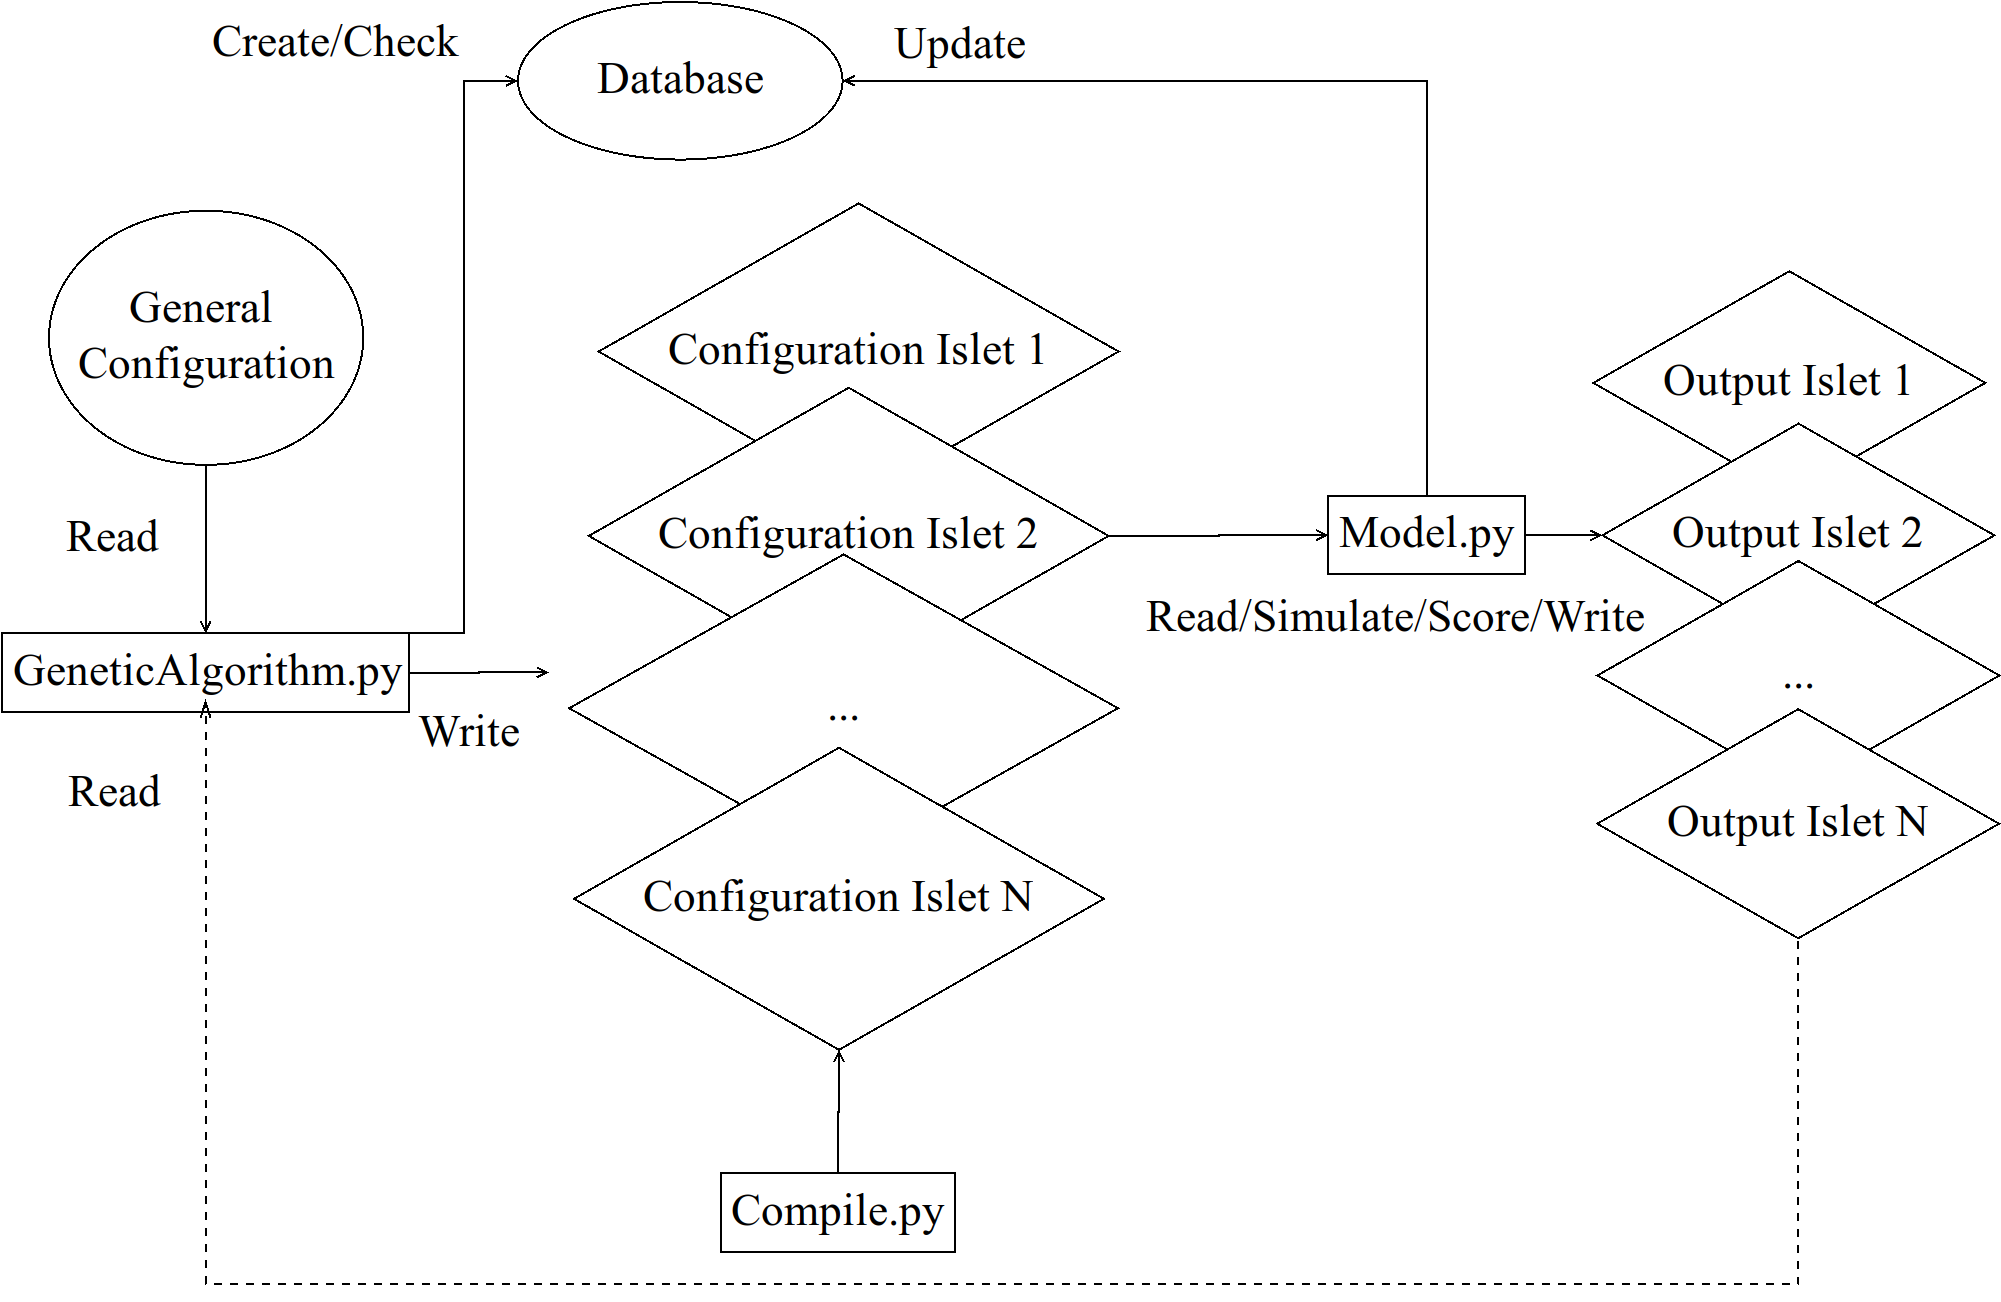
\includegraphics[scale=0.20]{Figures/architecture.png}
	\caption{Architecture of the evolutionary algorithm}
\end{figure}
The evolutionary algorithm is comprised of four recurrent steps: initialization, simulation, selection, and mutation. Initialization consisted of creating configuration files for each cell in an islet according to ranges within which model parameters were allowed to vary and setting up a folder in which appropriate current representations in nmodl would be stored and compiled. Simulation involved reading from the relevant configuration files, transferring control to NEURON to generate data for the given configuration, and scoring the data based on similarity to a reference data set (see the Scoring section). Selection involved passing the highest scoring subset of the current generation's islets to the next generation. The portion of subsequent generations subject to this non-random selection is determined at runtime, and the complementary random subset of the subsequent generation involved creating new configuration files instead of the more commonly used approach of randomly selecting parameters for models from the previous generation. This was done to compensate for the limited scoring metric by increasing randomization. Mutation then changed any parameter that was allowed to vary, randomly within its appropriate range with a probability determined at runtime.
\par Running simulations sequentially, especially with large population sizes and through many generations was significantly slower than running those simulations in parallel. For this reason, a logical structure for the evolutionary algorithm involved the parallelization of computation across simulations. Due to the previously mentioned concerns regarding memory and storage, this parallelization would have to occur with the periodic access to predetermined hardware resources offered by the slurm workload manager in a high performance computing environment. This presented the challenge of unpredictable start times and address spaces for individual simulations. In order for the genetic algorithm to step from one generation to the next, each model instance would have to update some persistent storage to signify its completion and make the relevant details accessible to some independently executed program. A sqlite database was updated to signify simulation completion and store some information regarding model outputs (i.e. score, number of cells, etc.) since the relevant information fit well into the relational model as relational algebra could be used to simplify data processing and organization. Pickle was used to serialize more intricate information regarding model score and comparisons to reference data.

\subsection{Scoring}
\begin{figure}[h!]\label{score}
	\begin{subfigure}{.33\textwidth}
		\centering
		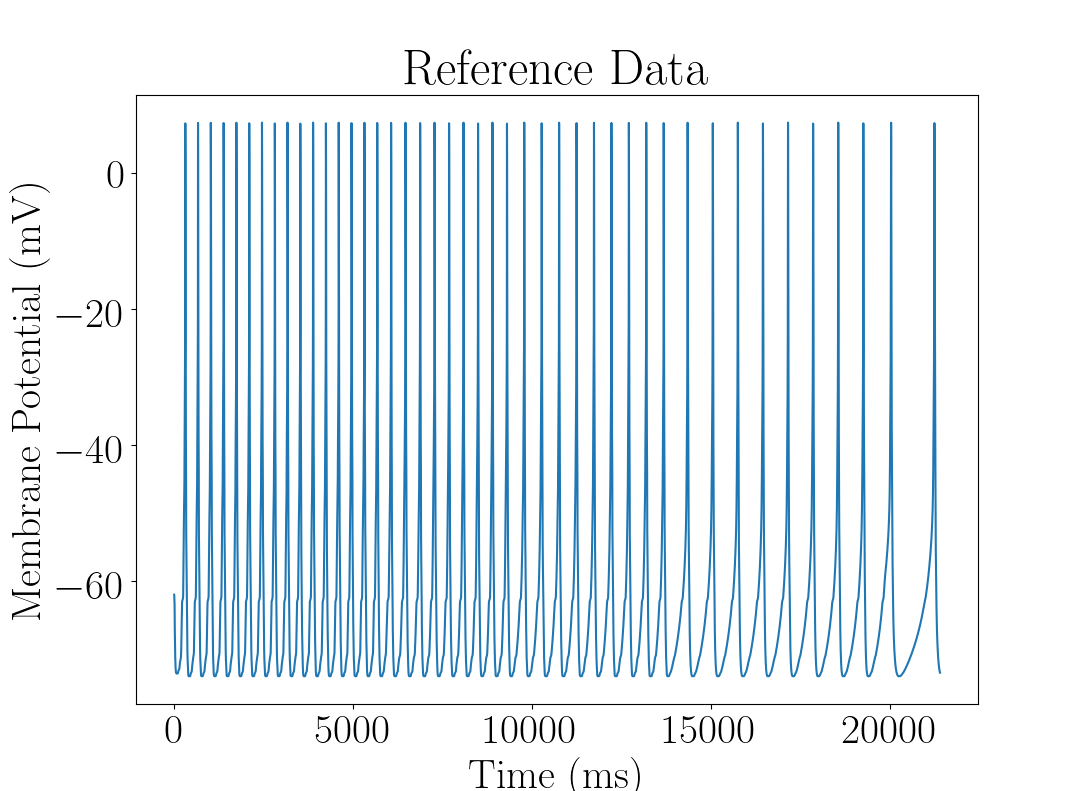
\includegraphics[scale=0.20]{Figures/reference.png}
		\caption{}
		\label{ref}
	\end{subfigure}
	\begin{subfigure}{.33\textwidth}
		\centering
		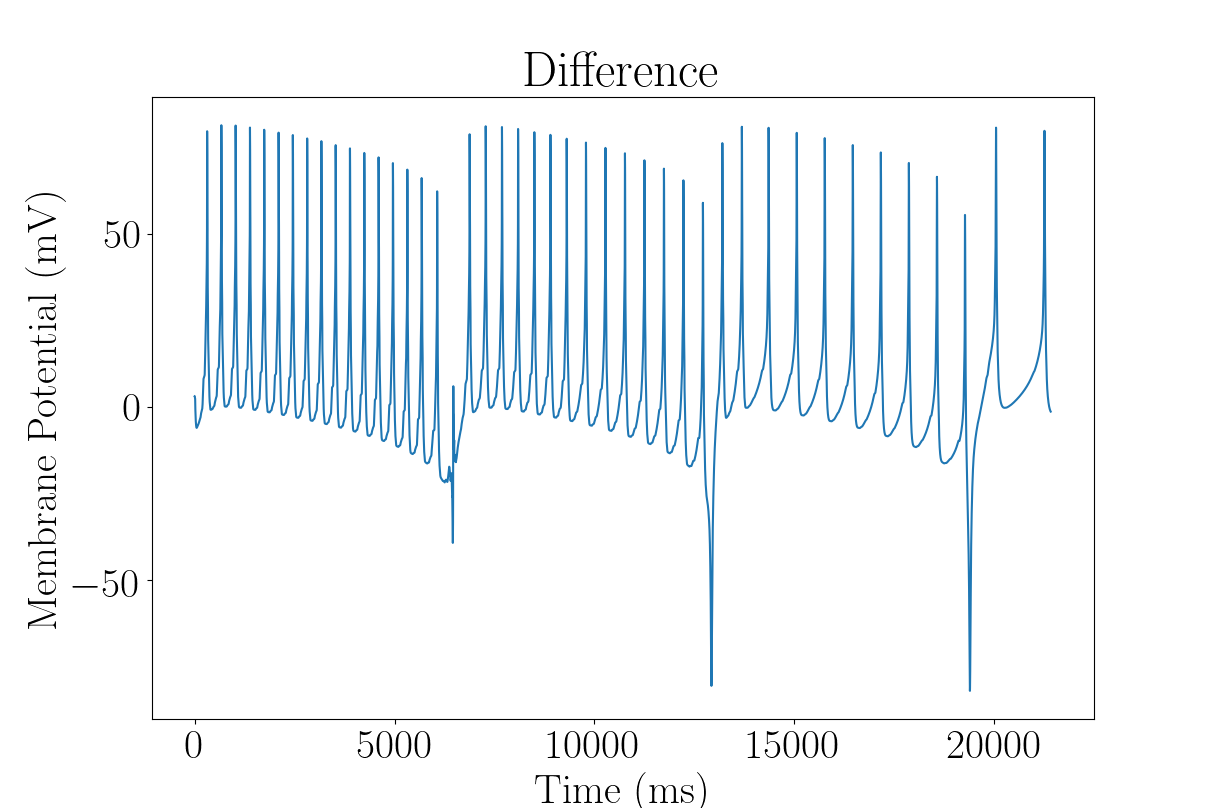
\includegraphics[scale=0.20]{Figures/difference.png}
		\caption{}
		\label{diff}
	\end{subfigure}
	\begin{subfigure}{.33\textwidth}
		\centering
		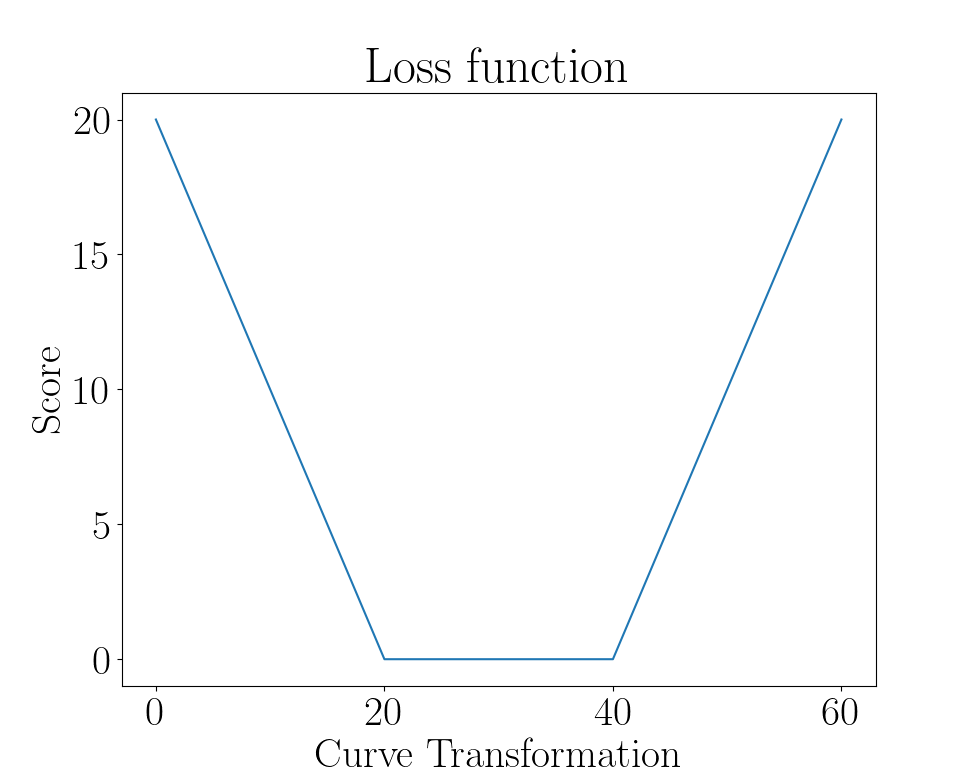
\includegraphics[scale=0.20]{Figures/loss.png}
		\caption{}
		\label{loss}
	\end{subfigure}%
	\caption{Scoring process}
\end{figure}
A strength of this computational model is the flexibility of the data set (i.e. sampling rate, duration, initial conditions) that can be used to parameterize it through the evolutionary algorithm. To best facilitate this flexibility, especially in a future use, the scoring metric and accompanying algorithm were kept simple in this implementation. The sole metric utilized was similarity in the membrane potential time series of simulated $\beta$ cells  to that of a reference data set. Both time series were adjusted such that the sampling rate and duration matched appropriately, and the difference was taken at each point in the simulation. 
\par The scoring process consists of three major steps. The membrane potential of each cell of an islet instance is first normalized to the same time scale that contained the reference data (figure 3a). A difference at each time step is taken between the two data sets and a new time series (figure 3b) is generated. This time series is compressed to a single value by summing all data points and this sum is put through a linear loss function with some threshold (figure 3c). A final sum was completed on the loss output of each compressed time series for each cell of an islet. These scores were compared to each other when instances were evaluated according to how well they reproduced data observed in biological islets. Values that may change the pool of islets selected from a generation (including the median, threshold, and rise of the loss function) were determined at runtime and were the same for all islet instances.

\section{Considerations}
This model is the first to represent the major cells of pancreatic islets within a full islet model. The use of an evolutionary algorithm to parameterize that model and quantify its accuracy was considered by at least one other paper with a similar scope, but this implementation remains unique among computational models of endocrine cells \cite{gurkiewicz_numerical_2007}. However, to produce meaningful data especially to clinicians and those involved in drug development, this model should be modified according to the conditions under which simulations occur, and the intentions of the researcher. This is especially true regarding modification of the scoring metric and accompanying selection criteria. For models which attempt to capture whole islet function, it is suggested that a multi-objective evolutionary algorithm which accounts for the fidelity of multiple variables (i.e. secretion, gating, etc.) for each cell type to distinct data sets be used in contrast to the single-object algorithm which only considered membrane potential in beta cells used in this thesis. It is worth noting that the focus of this thesis was the development of a framework on which future work will build and develop physiologically significant data. Therefore preliminary results are limited and were deemed not worth focusing on in this document.
\par We hope this model can provide the basis for a new class of computational models of pancreatic islets which view these clusters of endocrine cells as interdependent systems which are best understood through interactions between their spatial, physiological, and environmental profiles.
\clearpage

\clearpage
\printbibliography

\textbf{Github}: https://github.com/Tikahari/Model-of-Pancreatic-Islets/
\end{document}
